

En este capítulo se comentará el diseño de la arquitectura general, el
modelo de datos y también aspectos más concretos del diseño del servidor y la aplicación
móvil.



\section{Arquitectura}
La aplicación que estamos desarrollando seguirá la arquitectura
en tres capas. En este patrón arquitectónico cliente/servidor se diferencian tres
capas, una capa de interface de usuario , una capa de persistencia
y una capa intermedia llamada de servicios que permite la llamada de forma remota a la capa modelo(capa que contiene la lógica) por parte del cliente. Este esquema se puede apreciar en la Figura~\ref{fig:arquitectura2}. Este esquema esta compuesto por:




\begin{figure}
		\centering
		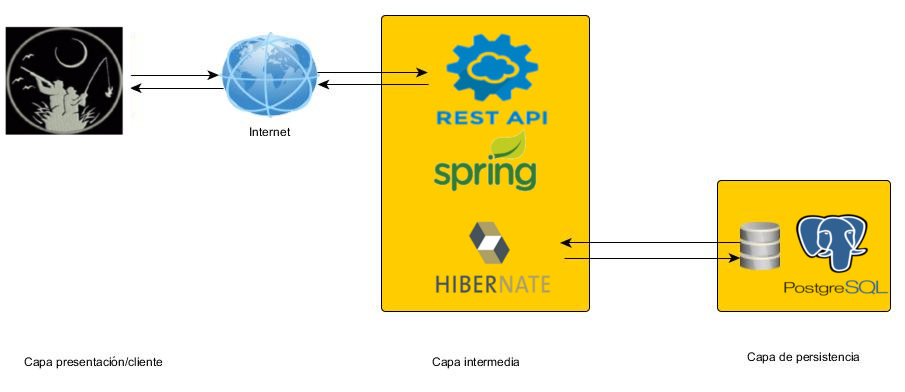
\includegraphics[width=\textwidth] {arquitectura2.png}
		\caption{Esquema general de la arquitectura del sistema }\label{fig:arquitectura2}
	\end{figure}


\begin{itemize}
\item \textbf{Capa de presentación/cliente}:\\
Capa que nos proporciona la información relacionada con los servicios que puede invocar el cliente. Es la encargada de comunicarse con las otras capas para guardar la información de cada usuario. En sí es la capa con la que va a interactuar el usuario cada vez trabaje con esta aplicación.

\item \textbf{Capa intermedia:}\\
Esta capa es la encargada de enlazar la capa de persistencia con la capa de presentación/cliente. Lo que hace es recoger los datos que provienen de la base de datos, necesarios para satisfacer el servicio invocado y enviárselos al cliente.

\item \textbf{Capa de persistencia:}\\
Esta capa es la encargada de almacenar los datos del sistema en la base de datos, además contiene todos los mecanismos de acceso a datos necesarios para poder hacer persistentes los datos.
 Esta capa debe ofrecer una interface que ayude a la comunicación con la capa intermedia, de manera que se abstraiga de la tecnología usada en el sistema de almacenamiento y no cree una dependencia con ella. Esta abstracción permitirá hacer cambios o actualizaciones en la tecnología sin afectar a otras capas con las que pudiera interaccionar en un futuro.\\
 


\end{itemize}
Una vez comentada la arquitectura general del sistema, pasaremos a comentar la capa intermedia un poco más a fondo ya que en ciertas ocasiones, la capa intermedia puede estar compuesta de N-capas(Arquitectura en N-capas). Esta es una de esas ocasiones.

Los servidores que siguen el modelo Modelo-Vista-Controlador consiguen separar los datos de la  aplicación, la lógica de negocio  y el envío  de información por la red.
Ésta separación ayuda al desarrollo de la aplicación tanto a la hora de crear la como a la hora de hacer su mantenimiento ya que marca al desarrollador a colocar el código en una capa concreta. \\


Los componentes capas que componen al patrón MVC son:

\begin{itemize}
\item \textbf{Modelo:}
Está compuesta por clases que tienen acceso a los datos ofreciendo unos métodos para ser usados de manera sencilla por las capas superiores. Éstos métodos son los encargados de acceder a la base de datos y proporcionar los datos persistentes.
\item \textbf{Vista:}
Está formada por el interfaz donde se realizan las llamadas entre el servicio web, peticiones HTTP en las que la información va en formato JSON, y la aplicación cliente.
\item \textbf{Controlador:}
Esta capa será la encargada de implementar la lógica del interface llamando a las operaciones que ofrece el modelo y seleccionando la vista asociada a cada petición.
\end{itemize}
\begin{figure}
		\centering
		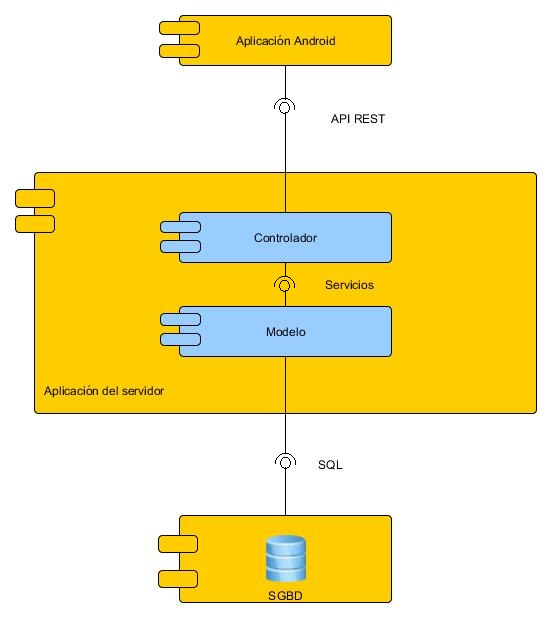
\includegraphics[width=\textwidth] {componentes.jpg}
		\caption{Diagrama de componentes del sistema }\label{fig:componentes}
	\end{figure}
 Esta descripción anteriormente reflejada representa a la siguiente Figura~\ref{fig:componentes}
\section{Capa de datos}
\begin{figure}[H]
		\centering
		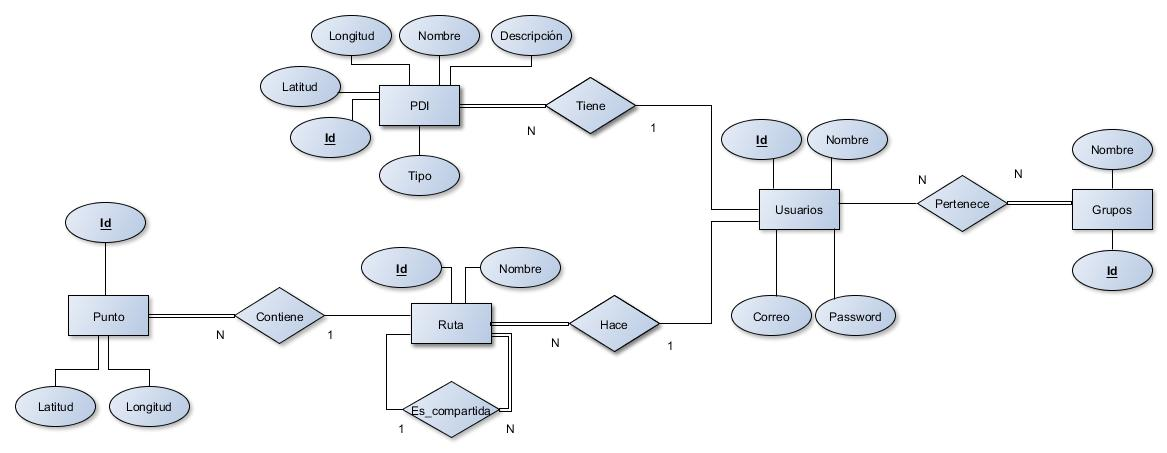
\includegraphics[width=\textwidth] {BD.jpg}
		\caption{Entidad relación  }\label{fig:BD}
	\end{figure}
	En la Figura~\ref{fig:BD} queda reflejado el modelo  entidad-relación de nuestro sistema. A continuación comentaremos el dominio.\\
La entidad principal sobre la que gira la aplicación es \textbf{Usuario}. Este puede crear \textbf{Grupos} a los que pasa a pertenecer al ser creados y los cuales desaparecen del sistema una vez que queden sin integrantes automáticamente.  El usuario puede crear \textbf{PDI(Puntos De Interés)} los cuales son propios y privados de un solo usuario con los atributos que aparecen reflejados en la figura. El usuario también puede realizar \textbf{Rutas} que a su vez pueden tener \textbf{Puntos} asociados a ellas, es decir, el  usuario crea una ruta asociándola a el y la ruta tiene asociada a ella puntos.
 Un caso especial serían las rutas compartidas asociadas a una principal, en las cuales el usuario crea una ruta y después la compartes con otros usuarios. Para  quedar esto reflejado en el entidad-relación tenemos la relación \textit{Asociada-a principal}.
	
\section{Servidor}
Para permitir una comunicación entre la aplicación del cliente y la capa de persistencia hemos desarrollado un servidor desplegado en un proveedor de servidores , al que se podrá acceder de manera remota y que permitirá tener acceso a las funcionalidades de la capa persistente. La arquitectura del servidor la podremos ver en la Figura~\ref{fig:arquitectura-servidor}

La solución mencionada anteriormente será un servidor, en java, que  usará Spring ya que facilita la creación de aplicaciones de forma cómoda y rápida.\\

Durante el desarrollo de este proyecto el servidor ha sido desplegado en un proveedor de servidores virtuales llamado 
  DigitalOcean, ya que ofrece distintos lugares donde poder ubicarlo. Hemos decidido hacerlo en uno concreto de Alemania para que el ping fuera más cercano y rápido.
\begin{figure}
		\centering
		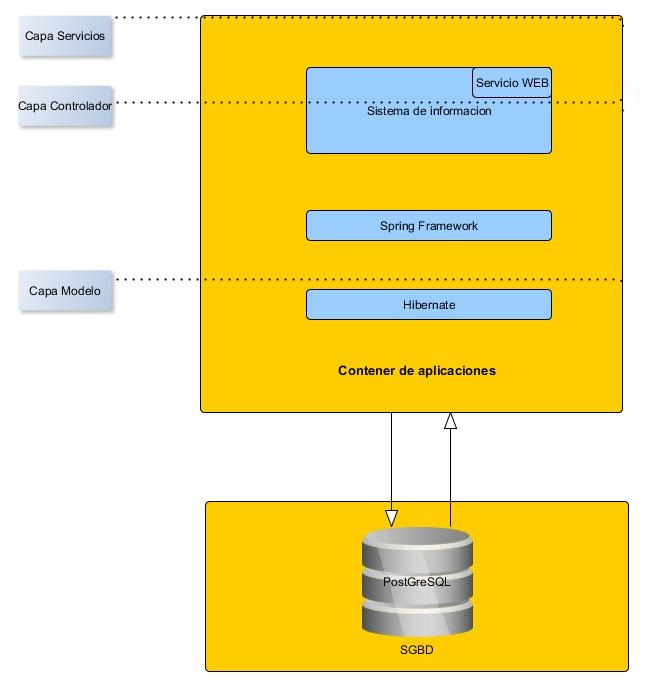
\includegraphics[width=\textwidth] {arquitectura-servidor.jpg}
		\caption{Arquitectura del servidor }
		\label{fig:arquitectura-servidor}
	\end{figure}


\subsection{Servicio web}
 La comunicación en esta capa se hará mediante una API. Una API describe la forma en que los programas o los sitios webs intercambian datos, cuyo formato  de intercambio de datos normalmente es JSON. En este servicio hemos decidido usar una API REST, un tipo de arquitectura de desarrollo web que se apoya totalmente en el estándar HTTP para la obtención de datos. A través de los siguientes peticiones podremos acceder a los distintos recursos.
 

\begin{itemize}
\item Los métodos de acceso indican la acción se queremos realizar sobre los recursos de nuestro sistema. Siguiendo esta línea tenemos el GET para solicitar un recurso pedido. POST para crear el recurso en el sistema y  para eliminar recursos usaremos DELETE. 



\item Dependiendo del método usado se irán cambiando la ruta en la petición HTTP y el contenido de ellas(cuerpo). Un POST tendrá una URL sencilla ya que los datos del objetos para ser creado irán en el cuerpo mientras que el GET y DELETE la tendrán de la forma \textit{ /usuario/{idusuario}} para obtener un objeto concreto o eliminarlo.





 


\end{itemize}

\subsection{Organizacion dos paquetes}
La aplicación del servidor sigue un arquetipo en 5 paquetes distintos de clases Java y uno para los test:
\subsubsection{java}
\begin{itemize}
\item\textbf{ es.udc.fi.dc.config} Contiene las clases Java de configuración de Spring.
\item \textbf{es.udc.fi.dc.model} Contiene todos los modelos de datos que estarán almacenados en la base de datos.
\item \textbf{es.udc.fi.dc.daos} Contiene los interfaces (JpaRepository) que aceden a los datos del sistema.
\item \textbf{es.udc.fi.dc.controller} Contiene las clases relacionadas  con las peticiones remotas.
\item  \textbf{es.udc.fi.dc.services} Contiene tanto los interfaces de los servicios como la implementación de los mismos.


\end{itemize}
\subsubsection{test}

\textbf{es.udc.fi.dc.test} Contiene las clases que realizan los test.
\subsection{Transmisión de la información}
Como se mencionó anteriormente para el servicio web usaremos la API REST, esta necesita un lenguaje de intercambio para la transmisión de información. El formato que seguiremos para la transmisión será el JSON y como parseador Jackson.
JSON, siglas JavaScript Object Notation, es un formato estándar de transmisión de la información muy cómodo de usar que emplea pares de clave-valor. 	Ejemplo de Json en la Figura~\ref{fig:json}
	\begin{figure}
		\centering
		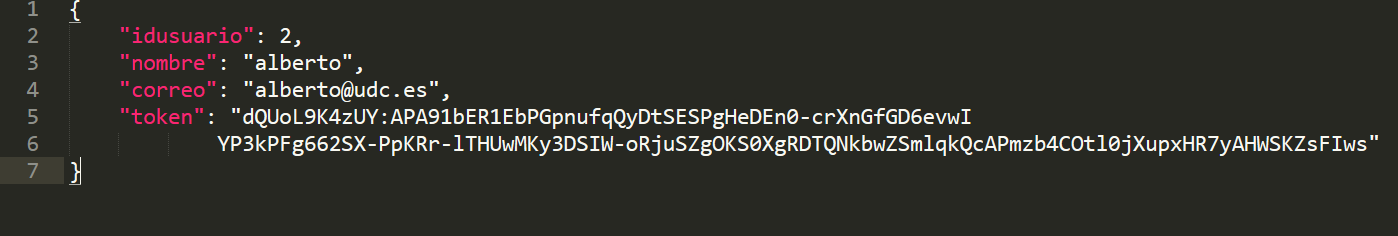
\includegraphics[width=\textwidth] {json.PNG}
		\caption{JSON }
		\label{fig:json}
	\end{figure}
\subsection{Gestión de las clases persistentes}
Para gestionar las clases persistentes de nuestra aplicación usaremos el patrón de diseño basado en DAO(Data Access Object).

 Un DAO define un interfaz que contiene conjunto de operaciones de persistencia y a su vez una implementación permitiendo la gestión de las entidades en la base de datos. Es decir oculta la gestión de la base de datos y a su vez la tecnología que usamos en ella, dotando a cada clase persistente de un DAO asociado a ella. En éste proyecto hemos usado Spring Data JPA que nos proporciona una interfaz para la gestión de los objetos del dominio sin tener que escribir nosotros la implementación de los métodos. Esto nos permite ganar agilidad a la hora de crear los DAOs ya que permite extender esta interfaz a nuestra clase DAO proporcionando todos los métodos CRUD, métodos para modificar o eliminar objetos de ese tipo. Éste interfaz se llama JpaRepository.\\


Otro motivo por el cual usamos JpaRepository es que permite extender la creación de una buena serie de métodos de búsqueda por el nombre de los atributos de nuestras clases persistentes simplemente definiendo los como un método de nuestro interfaz del DAO.
	
	
	
	
	
\begin{lstlisting}[language=java,caption={JpaRepository},label=DescriptiveLabel]
    
public interface UsuarioRepository 
	extends JpaRepository<Usuario, Long> {

	public Usuario findByCorreo(String correo);

	public Usuario findByNombre(String nombre);

	public List<Usuario> findByNombreContaining
		(String nombre);

	@Override
	public <S extends Usuario> S save(S usuario);

	@Override
	public void delete(Long idUsuario);

	@Override
	public boolean exists(Long idUsuario);

	@Override
	public <S extends Usuario> S saveAndFlush(S usuario);

	@Override
	public Usuario findOne(Long idUsuario);
	}


\end{lstlisting} 
	
	
	
	
\section{Aplicación Móvil}
La capa de presentación será accesible por el usuario a través de una aplicación móvil desarrollada en Android. Los aspectos más relevantes serán expuestos a continuación.

\subsection{Servicios}
\begin{itemize}
\item \textbf{Google Maps API}. Es un servicio web proporcionado por google que nos permite usar los mapas en nuestras aplicaciones y también conocer la ubicación del usuario  en todo momento. Esta ubicación la marca con un punto azul pero no suministra coordenadas(latitud y longitud).
\item \textbf{Google Location}. Es un servicio de google que nos suministra las coordinadas del usuario, según varía la posición ciertos metros o cada cierto tiempo.
\item \textbf{Rest SystemService}. Este punto sería el que ejecuta nuestro propio servidor para guardar o devolver lo datos de los usuario, puntos de interés, rutas o grupos del usuario.
\item \textbf{Firebase Cloud Messaging} Firebase Cloud Messaging (FCM) es una solución de mensajería multiplataforma que te permite enviar mensajes de forma segura y gratuita. En este caso lo hemos utilizado para enviar notificaciones push cuando se inicia una ruta compartida.
\end{itemize}
\begin{figure}[H]
		\centering
		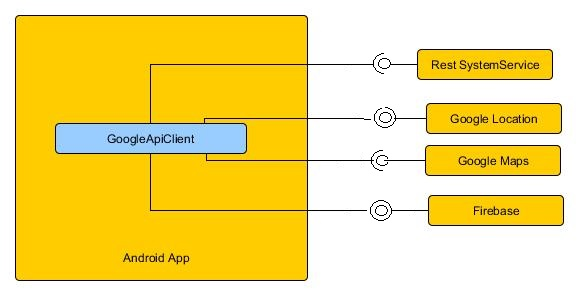
\includegraphics[width=\textwidth] {arquitectura-movil.jpg}
		\caption{Servicios de la aplicación móvil }
		\label{fig:arquitectura-movil}
	\end{figure}
	
	
\subsection{Organización de los paquetes}
La organización seguida en la aplicación móvil es la de agrupar las clases por funcionalidades comunes.
\begin{itemize}
\item  \textbf{com.example.alberto.hunter-android.activities}, contiene todas las actividades.
\item \textbf{com.example.alberto.hunter-android.adapter}, contiene los adaptadores.
\item \textbf{com.example.alberto.hunter-android.model},contiene todos los modelos de datos.
\item \textbf{com.example.alberto.hunter-android.utils}, contiene las clases auxiliares.\\ 

Con esta organización por funcionalidades comunes creamos un proyecto claro y  organizado lógicamente.

\end{itemize}


